\documentclass[12pt, a4paper]{article}
\usepackage{amsmath}
\usepackage{amsfonts}
\usepackage{amsthm}
\usepackage{mathtools}
\newtheorem{theorem}{Theorem}[section]
\newtheorem{definition}{Definition}[section]
\numberwithin{equation}{section}
\usepackage{pgfplots}
\pgfplotsset{width=10cm,compat=1.9}
\graphicspath{ {img/} }
\DeclareGraphicsExtensions{.png}

\title{Text retrieval}
\author{Kristian Wichmann}

\begin{document}
\maketitle

\section{Information retrieval vs. text retrieval}
\textit{Information retrieval} (IR) is the process of obtaining information from a source of relevant data. Very often, we will think of digital systems, and hence the amounts of data involved are very large. In general, we could be looking for any kind of information, like pictures, audio, or video.

\textit{Text retrieval} (TR) is the subset of IR which deals with text. The most iconic example is web search based on a text query, like the services provided by search engines such as Google and Bing.

\section{Push and pull modes of text access}
Text retrieval happens in two major modes: push and pull.

\subsection{Push mode}
In push mode, the text is suggested (pushed) to the user based on previous interactions. This is what typically happens in a recommender system. For instance, Netflix will suggest movies and series based on your view history.

\subsection{Pull mode}
In pull mode, the user takes the initiative to get (pull) the text. This may be further subdivided:
\begin{itemize}
\item\textit{Querying} - Here, the user knows what to look for, at enters a keyword text: a query. This works well when the user knows what he/she is looking for.
\item\textit{Browsing} - Here, the user navigates through the data, following a path enabled by its structure. This works well when the user wants to explore the data.
\end{itemize}
We will focus on querying in this document.

\section{Terminology}
Here we describe the various ingredients needed to make a \textit{retrieval model}:
\begin{itemize}
\item We work with a \textit{vocabulary} $V=\{w_1,\cdots,w_N\}$ of words.
\item A \textit{query} $q$ may be written $q=(q_1,\cdots,q_m)$, where $q_i\in V$.
\item A \textit{document} can be written $d_i=(d_{i1},\cdots,d_{im_i})$.
\item A \textit{collection} of documents is $C=\{d_1,\cdots,d_M\}$.
\end{itemize}

\subsection{Term frequency-inverse document frequency}
A given vocabulary word $w\in V$ can be described in terms of its appearence in a document/collection. Two common measures are \textit{term frequency} (tf) and \textit{inverse document frequency} (idf).

\subsubsection{Term frequency}
Term frequency directly describes the occurrence of $w$ in $d$. There's many variations of this. The simplest two are:
\begin{itemize}
\item 0 or 1 depending on whether w is present or not.
\item Raw frequency $\textrm{tf}(f,d)$. A count of the number of occurences.
\end{itemize}
Later we will look at transformations of tf.

\subsubsection{Inverse document frequency}
The inverse document frequency describes how unusual a word $w$ is in a collection $C$. If $n_{wC}$ is the number of documents in $C$ which contains $w$, the idf is defined as:
\begin{equation}
\textrm{idf}(w,C)=\log\frac{N+1}{n_{wC}}
\end{equation}
To avoid division by zero for non-occuring $w$, 1 is sometimes added to the denominator. A number of different weighting schemes for idf exists, but this is the one we will primarily use here.

\begin{figure}
\centering
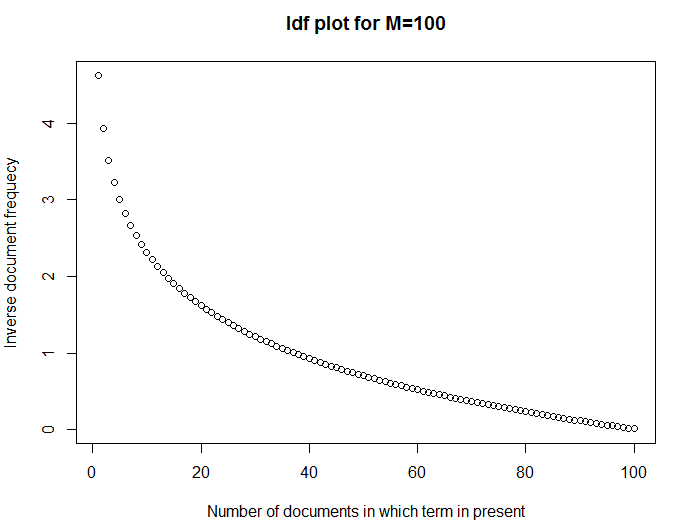
\includegraphics[width=0.75\textwidth]{idf_plot}
\caption{An example idf plot.}
\label{fig:idf_plot}
\end{figure}

Figure \ref{fig:idf_plot} shows an example of how idf decreases with higher document occurrences.

\section{The text retrieval problem}
Given a query $q$, we wish to extract the set of \textit{relevant documents} $R(q)\subseteq C$ for the query.

In practice, all we can hope for is an approximation of the relevant documents: $R'(q)$.

\section{Strategies}

\subsection{Document selection strategies}
One way to solve the text retrieval system is to build a binary classifier $f$, which given a document $d$ and a query $q$ returns either 0 or 1, depending on whether or not $d\in R'(q)$:
\begin{equation}
R'(q)=\{d\in C|f(d,q)=1\}
\end{equation}
Of course, any way to choose $R'(q)$ is technically a binary classifier, but the idea is that $f$ decides the \textit{absolute relevance} of the document - there is no further nuance beyond "yes" or "no".

With this strategy, there's $2^N$ possible different outcomes, since each document is either relevant or not.

\subsection{Document ranking}
Instead, the function $f$ might have a continuum of real values instead of just $\{0, 1\}$. Then we might choose $R'(q)$ based on a \textit{cutoff} $\theta$:
\begin{equation}
R'(q)=\{d\in C|f(d,q)>\theta\}
\end{equation}
Here $f$ is more nuanced, and decides what is called the \textit{relative relevance} of the document. A list of documents sorted by decreasing relevance could be constructed, and $\theta$ decides where to stop the list. Or rather, if the user browses such a list, $\theta$ is decided by the user.

There's $N!$ different possible outcomes with this strategy, since each ordering of documents is distinct.

\subsubsection{The probability ranking principle}
The document ranking strategy is (under certain conditions) guaranteed by the \textit{probability ranking principle} (PRP) to be of optimal utility to the user.

\section{Vector space model}
One approach to building a selection function is to use a \textit{vector space model}. This is a \textit{similarity-based} model, as it tries to give a measure of how similar the query and a document is.

\subsection{The bag of words model}
In the \textit{bag of words} model (BOW), we disregard the ordering of the words in a document, and simply see them as an unordered list. Clearly, some information is lost in this simplification, but sometimes it will still yield useful results. The vector space model uses BOW.

\subsection{Types of vectors - simplest approach}
I each of the following cases, the relevant vector space for the model has a dimension of the size of the vocabulary $V$. In other words is has $N$ dimensions.

\subsubsection{Bit vectors}
Here, each coordinate can only take on the values 0 or 1, indicating whether or not the word $w_i$ is present in the query/document or not.

\subsubsection{Frequency vector}
Going a bit further than bit vectors, here coordinate $i$ represents the number of times $w_i$ appears in the document.

\subsection{Similarity measure}
No matter which model is used, the simplest similarity measure between a query and a document (or between two documents) is the dot product between the two:
\begin{equation}
\textrm{similarity}=q\cdot d
\end{equation}
For bit vectors this is equal to the distinct number of query terms matched in the document. For frequency vectors, it is the total count of occurrences of any query term in the document.

\subsection{Including idf: tf-idf weight vector}
The vector types mentioned above doesn't take into account how commonly used a word is. For instance, occurences of the words "the", "a" or "is" have the same impact on the similarity score than more specific terms. Some kind of \textit{weighting} is needed.

One approach, it to use the inverse document frequency, since it will be low for common words. In other words, the vector coordinate for the word $w$ should be the frequency of the words in $d$ times the idf for the word in the relevant collection $C$. In other words it is:
\begin{equation}
\textrm{tf}(w,d)\cdot\textrm{idf}(w,C)
\end{equation}
Because of this, it is known as the \textit{tf-idf weight vector}.

\subsection{Tf transformation: BM25}
To simply have the raw tf count in the formula above is also problematic. It rewards simple repetition of a given term too much; the first occurence of a search term is valued as highly as the fiftieth. In order to remedy this, we need to perform some transformation $t$ of tf.

We've already seen one such transform when we considered the binary representation of whether a term is present or not. Here, the transformation is:
\begin{equation}
t(\textrm{tf})=
\begin{cases}
0 & \textrm{when }\textrm{tf}=0 \\
1 & \textrm{otherwise}
\end{cases}
\end{equation}
For this purpose however, it is too drastic. A better looking option is a logarithmic transformation:
\begin{equation}
t(\textrm{tf})=\log(1+\textrm{tf})
\end{equation}
Or even a nested logarithm:
\begin{equation}
t(\textrm{tf})=\log(1+\log(1+\textrm{tf}))
\end{equation}
However, it turns out that in many cases what works best is a transformation of the following type:
\begin{equation}
t(\textrm{tf})=\frac{(k+1)\textrm{tf}}{\textrm{tf}+k}
\end{equation}
This is known as a \textit{BM25 transformation}. Figure \ref{fig:bm25} shows this transformation for various $k$ values.

\begin{figure}
\centering
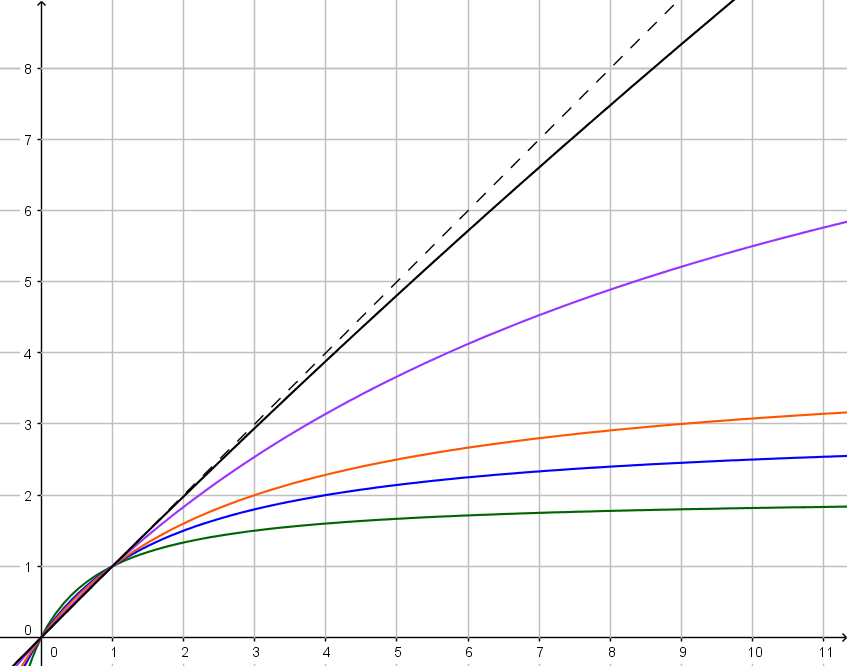
\includegraphics[width=0.75\textwidth]{bm25}
\caption{The BM25 transformation for $k=2, 3, 4, 10$ and $100$ respectively. The asymptote $x=k+1$ is not clear from this plot.}
\label{fig:bm25}
\end{figure}

\subsection{Taking document length into account}
Longer documents will usually include more words. Therefore, they will tend to get higher vector coordinates simply because of length. We may attempt to rememdy this by introducing a length \textit{normalization}.

We will require this normalization function to be 1 at average document length for $C$, a number we will denoted $\textrm{avdl}$. This may be accomplished by the following linear function:
\begin{equation}
n(l)=1-b+b\frac{l}{\textrm{avdl}}
\end{equation}
For $b>0$ this function grows larger for large document sizes, which is what we're looking for, since we want to divide by $n(d)$.

\section{Term-Frequency Matrix}
The chosen weights can be collected in what is known as the \textit{term-frequency matrix} (TFM). The name refers to frequency vectors, but it can be used for any weighting scheme. 

In the TFM, words from the vocabulary are in the $x$-direction, while documents from the corpus are in the $y$-direction. An example will make this clearer.

\subsection{Example of TFM}
Consider a corpus consisting of the following three text files:
\begin{enumerate}
\item "this is good"
\item "this is bad"
\item "this is very very bad"
\end{enumerate}
Here, the vocabulary consists of the following five words: this, is, good, bad and very. The corresponding TFM (using the frequency vector weight scheme) is shown in table \ref{table:TFM}.

\begin{table}[t]
\centering
\label{table:TFM}
\begin{tabular}{c|c|c|c|c|c|}
\cline{2-6}
\multicolumn{1}{l|}{Docoment/Word} & \multicolumn{1}{l|}{\textbf{this}} & \multicolumn{1}{l|}{\textbf{is}} & \multicolumn{1}{l|}{\textbf{good}} & \multicolumn{1}{l|}{\textbf{bad}} & \multicolumn{1}{l|}{\textbf{very}} \\ \hline
\multicolumn{1}{|c|}{\textbf{1}}   & 1                                  & 1                                & 1                                  & 0                                 & 0                                  \\ \hline
\multicolumn{1}{|c|}{\textbf{2}}   & 1                                  & 1                                & 0                                  & 1                                 & 0                                  \\ \hline
\multicolumn{1}{|c|}{\textbf{3}}   & 1                                  & 1                                & 0                                  & 1                                 & 2                                  \\ \hline
\end{tabular}
\caption{TFM example}
\end{table}

\subsection{Abstract form}
Note how in the example each row is a document vector. In other words, the TFM could abstractly be written as:
\begin{equation}
\begin{pmatrix}
\textrm{---} & d_1^T & \textrm{---} \\
\vdots & \vdots & \vdots \\
\textrm{---} & d_M^T & \textrm{---}
\end{pmatrix}
=
\begin{pmatrix}
| & \cdots & | \\
d_1 & \cdots & d_M \\
| & \cdots & |
\end{pmatrix}^T
\end{equation}
Here $d_i$ is the column vector for document $i$.

\subsection{Inverted index}
The \textit{inverted index} form of the TDM, is basically the same data, but viewed columnwise: For instance, from the fourth column in the example above, we can immediately infer that the word "bad" appears once in documents 2 and 3. This is much quicker than scanning through the entire corpus for the word.

Since in general, the TFM matrix will be rather sparse, different compression schemes for the inverted index are often used in practice.


\end{document}